% How to tell they don't know what they're doing.
% 1. \\, \vspace, \par
% 2. long, unused packages called in preamble. (amsfonts)
% 3. recreate standard solutions to common problems (use CTAN)


% Tips:
% 1. mini page side by side pages on the the same pdf page

% \begin{minipage}
% blah
% \end{minipage}
% \begin{minipage}
% blah
% \end{minipage}

% 2. Figures and tables

% 3. Unbreakable text use \mbox{texttext} no hyphen applied
%   the ~ character is also an unbreakable character

% 4. Tabbing environment used to set tab length
%   Set tab with \= stuff \= foo \\
%   \> more \> things

% UNDERSTANDING THE TABBING ENVIRONMENT
% learning how to make \= a tabbing \= environment \= \\
% this \> was \> hard to learn. \\
% Learning the hard way is my speciality \>\> \\
% \> Ima kill this line \> \kill
% \> Ima unkill this line \> \\
% m\=aking a new \= tabbing environment here now ok? \= ok. \\
% this \> was \> hard to learn. \> for me\\
% Learning the hard way is my speciality \>\> bam \> boozld \\
% \> Ima kill this line \> \kill \\
% \> Ima unkill this line \>

\documentclass{article}

\usepackage[margin=1in]{geometry}

\usepackage{amsmath,amssymb}

\usepackage{graphicx, tikz, tikz-3dplot, wrapfig}

\usepackage{fontspec}
\setmainfont{Courier Prime Code.ttf}

\title{Assignment 9: Exercise 1}
\author{Cameron Fredrickson}
\date{}

\begin{document}

\maketitle

\begin{tabbing}
col1 \= column 2 is this long \= column 3 is this longgggggggg \= column 4 is this long \kill \\
\> (a) $\displaystyle{\sum_{\substack{x+y+z=n \\ x,y,z\geq0}}}{xyz}$ \> (b) $\displaystyle{\overbrace{\alpha + \beta + \gamma + \delta}^{\text{this equals 3}} + \underbrace{a + b + c + d}^{\text{this equals 4}}}$ \> (c) $\displaystyle{x^n + y^n \overset{\text{?}}{=} z^n \text{ for } x, y, z \in \mathbb{Z}}$
\end{tabbing}

\begin{figure}[h!]
    \begin{minipage}[t][5cm][b]{0.5\textwidth}
        \begin{center}
            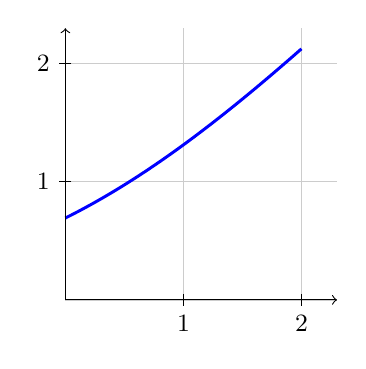
\begin{tikzpicture}[scale = 1.5]

            \draw [black!20, very thin] (0,0) grid (2.3,2.3);
            \draw [domain=0:2, smooth, line width = .25ex, blue, samples = 100] plot (\x, {ln(1+exp(\x))});
            \draw [->, thin] (0,0) -- (0,2.3);
            \draw [->, thin] (0,0) -- (2.3,0);
            \foreach \x in {1,2} {
              \draw (.05, \x) -- (-.05, \x) node [left] {\begin{small}$\x$\end{small}};
            }
            \foreach \x in {1,2} {
              \draw (\x, .05) -- (\x, -.05) node [below] {\begin{small}$\x$\end{small}};
            }
            \end{tikzpicture}
            \caption{Graph of $\log (1 + e^x)$}
        \end{center}
    \end{minipage}
    \begin{minipage}[t][5cm][b]{0.5\textwidth}
        \begin{center}
            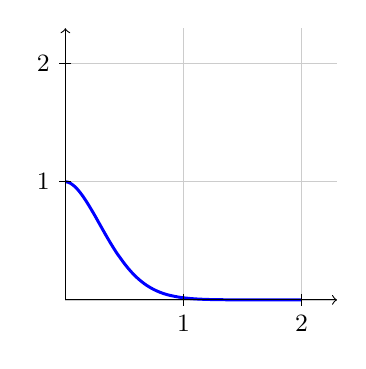
\begin{tikzpicture}[scale = 1.5]

            \draw [black!20, very thin] (0,0) grid (2.3,2.3);
            \draw [domain=0:2, smooth, line width = .25ex, blue, samples = 100] plot (\x, {pow(sin(\x), pow(\x, 2))});
            \draw [->, thin] (0,0) -- (0,2.3);
            \draw [->, thin] (0,0) -- (2.3,0);
            \foreach \x in {1,2} {
              \draw (.05, \x) -- (-.05, \x) node [left] {\begin{small}$\x$\end{small}};
            }
            \foreach \x in {1,2} {
              \draw (\x, .05) -- (\x, -.05) node [below] {\begin{small}$\x$\end{small}};
            }
            \end{tikzpicture}
            \caption{Graph of $\sin^{x^2} x$}
        \end{center}
    \end{minipage}
\end{figure}

\begin{wrapfigure}{c}{1\textwidth}
    \begin{center}
        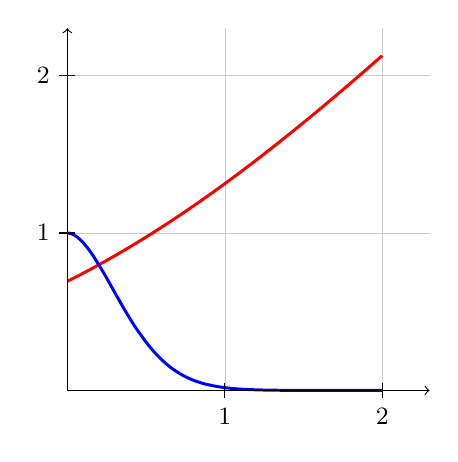
\begin{tikzpicture}[scale = 2]

        \draw [black!20, very thin] (0,0) grid (2.3,2.3);
        \draw [domain=0:2, smooth, line width = .25ex, red, samples = 100] plot (\x, {ln(1+exp(\x))});
        \draw [domain=0:2, smooth, line width = .25ex, blue, samples = 100] plot (\x, {pow(sin(\x), pow(\x, 2))});
        \draw [->, thin] (0,0) -- (0,2.3);
        \draw [->, thin] (0,0) -- (2.3,0);
        \foreach \x in {1,2} {
          \draw (.05, \x) -- (-.05, \x) node [left] {\begin{small}$\x$\end{small}};
        }
        \foreach \x in {1,2} {
          \draw (\x, .05) -- (\x, -.05) node [below] {\begin{small}$\x$\end{small}};
        }
        \end{tikzpicture}
    \end{center}
    \caption{$\sin^{x^2} x$ and $\log (1 + e^x)$ together on the same graph}
\end{wrapfigure}

\end{document}